\documentclass[10pt, compress]{beamer}

\usetheme{glasgow}

\usepackage{booktabs}
\usepackage[scale=2]{ccicons}
\usepackage{minted}

\usepgfplotslibrary{dateplot}

\usemintedstyle{trac}

% Specifiy the location of images to be used
\graphicspath{{src/}}

%% Customisation
% \newcommand{\V}[1]{\v} % vectors \v{c}
% \renewcommand{\v}[1]{\mathbf{#1}} % vectors
\newcommand{\ti}[1]{\tilde{#1}} % spectral representation
\newcommand{\tnsr}[1]{\underline{\underline{#1}}}

% Symbols
\renewcommand{\O}{\omega}  % omega
\newcommand{\E}{\varepsilon}  % epsilon
\renewcommand{\u}{\mu}  % mu
\newcommand{\p}{\rho}  % rho
\newcommand{\x}{\times}  % times
\renewcommand{\inf}{\infty}  % infinity
\newcommand{\infint}{\int\limits_{-\inf}^\inf} % integral by R
\newcommand{\e}{\mathrm{e}} % Straight-up exponential
\renewcommand{\j}{{j}\mkern1mu} % Straight-up exponential
\newcommand{\iu}{\mathrm{i}\mkern1mu}

\newcommand\ddfrac[2]{\frac{\displaystyle #1}{\displaystyle #2}}





\title{High Frequency Communication Systems}
\subtitle{Lecture 3}
\date{Spring 2021}
\author{Hasan T Abbas \& Qammer H Abbasi}
% \institute{}

\begin{document}

\maketitle

%%%%%%%%%%%%%%%%%%%%%%%%%%%%%%%%%%%%%%%%%%
%%%%%%%%%%%%%%%%%%%%%%%%%%%%%%%%%%%%%%%%%%
%%%%%%%%%%%%%%%%%%%%%%%%%%%%%%%%%%%%%%%%%%
\begin{frame}[fragile]
  \frametitle{Lecture Outline}
\begin{outline}[itemize]
  \1 Antennas and Radiation
  \1 Potential Functions
  \1 Antenna Characteristics
\end{outline}
\end{frame}
%%%%%%%%%%%%%%%%%%%%%%%%%%%%%%%%%%%%%%%%%%
%%%%%%%%%%%%%%%%%%%%%%%%%%%%%%%%%%%%%%%%%%
%%%%%%%%%%%%%%%%%%%%%%%%%%%%%%%%%%%%%%%%%%
\begin{frame}[fragile]
\frametitle{Sources of Electromagnetic Fields}
\begin{outline}
  \1 A distribution of currents and charges can generate and \color{red}{radiate} electromagnetic fields
    \2 The distribution is typically localised in a region of space
    \2 As an example, a simple wire can act as an \textit{antenna}
  \1 We are interested in determining the electromagnetic fields in space, given a current distribution
\end{outline}
\end{frame}

\begin{frame}
  \frametitle{Antenna}
  \begin{columns}[T] % align columns
  \begin{column}{.4\textwidth}
\begin{outline}
  \1 Antennas are most widely used for wireless communications
  \1 Modern antenna invention is attributed to Heinrich Hertz (1887)
  \2 Radio system was developed by Guglielmo Marconi (1897)
  \1 Due to the \textit{duality} principle, an antenna can also act as a receiver to EM radiation
\end{outline}
   \end{column}
 \begin{column}[T]{.6\textwidth}
    \begin{figure}
      \centering
          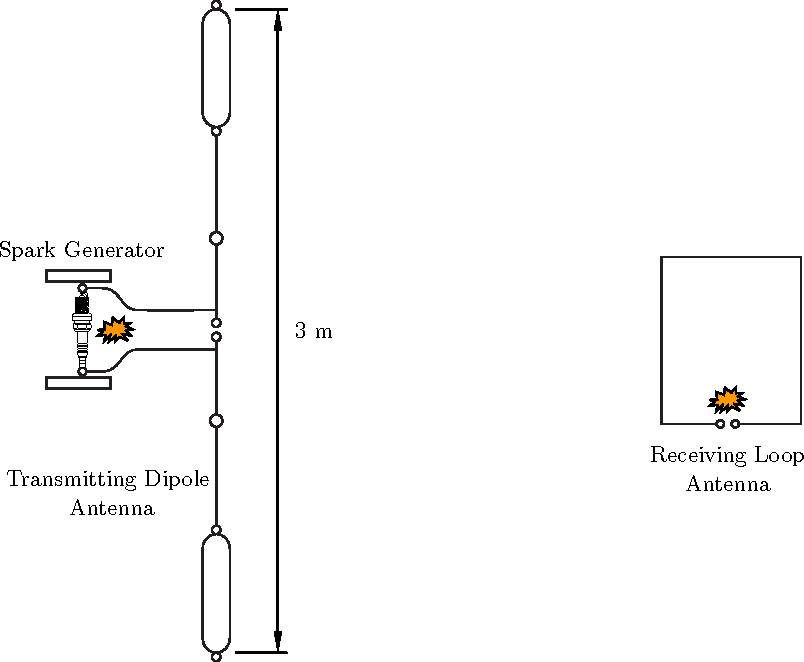
\includegraphics[width=.9\textwidth]{antenna_hertz.pdf}
      \caption{The Hertz's invention}
    \end{figure}
      \end{column}%
\end{columns}
  \end{frame}

\begin{frame}
  \frametitle{How Antennas Radiate}
    \begin{columns}[T] % align columns
  \begin{column}{.4\textwidth}
\begin{outline}
  \1 We need a \color{red}{disturbance} in the EM fields
  \2 Most commonly, this is caused by a time-varying electric current
  \1 The disturbance also depends on the nature of the antenna
  \2 For a wire antenna, the discontinuities at the ends cause radiation
\end{outline}
   \end{column}
 \begin{column}[T]{.6\textwidth}
    \begin{figure}
      \centering
          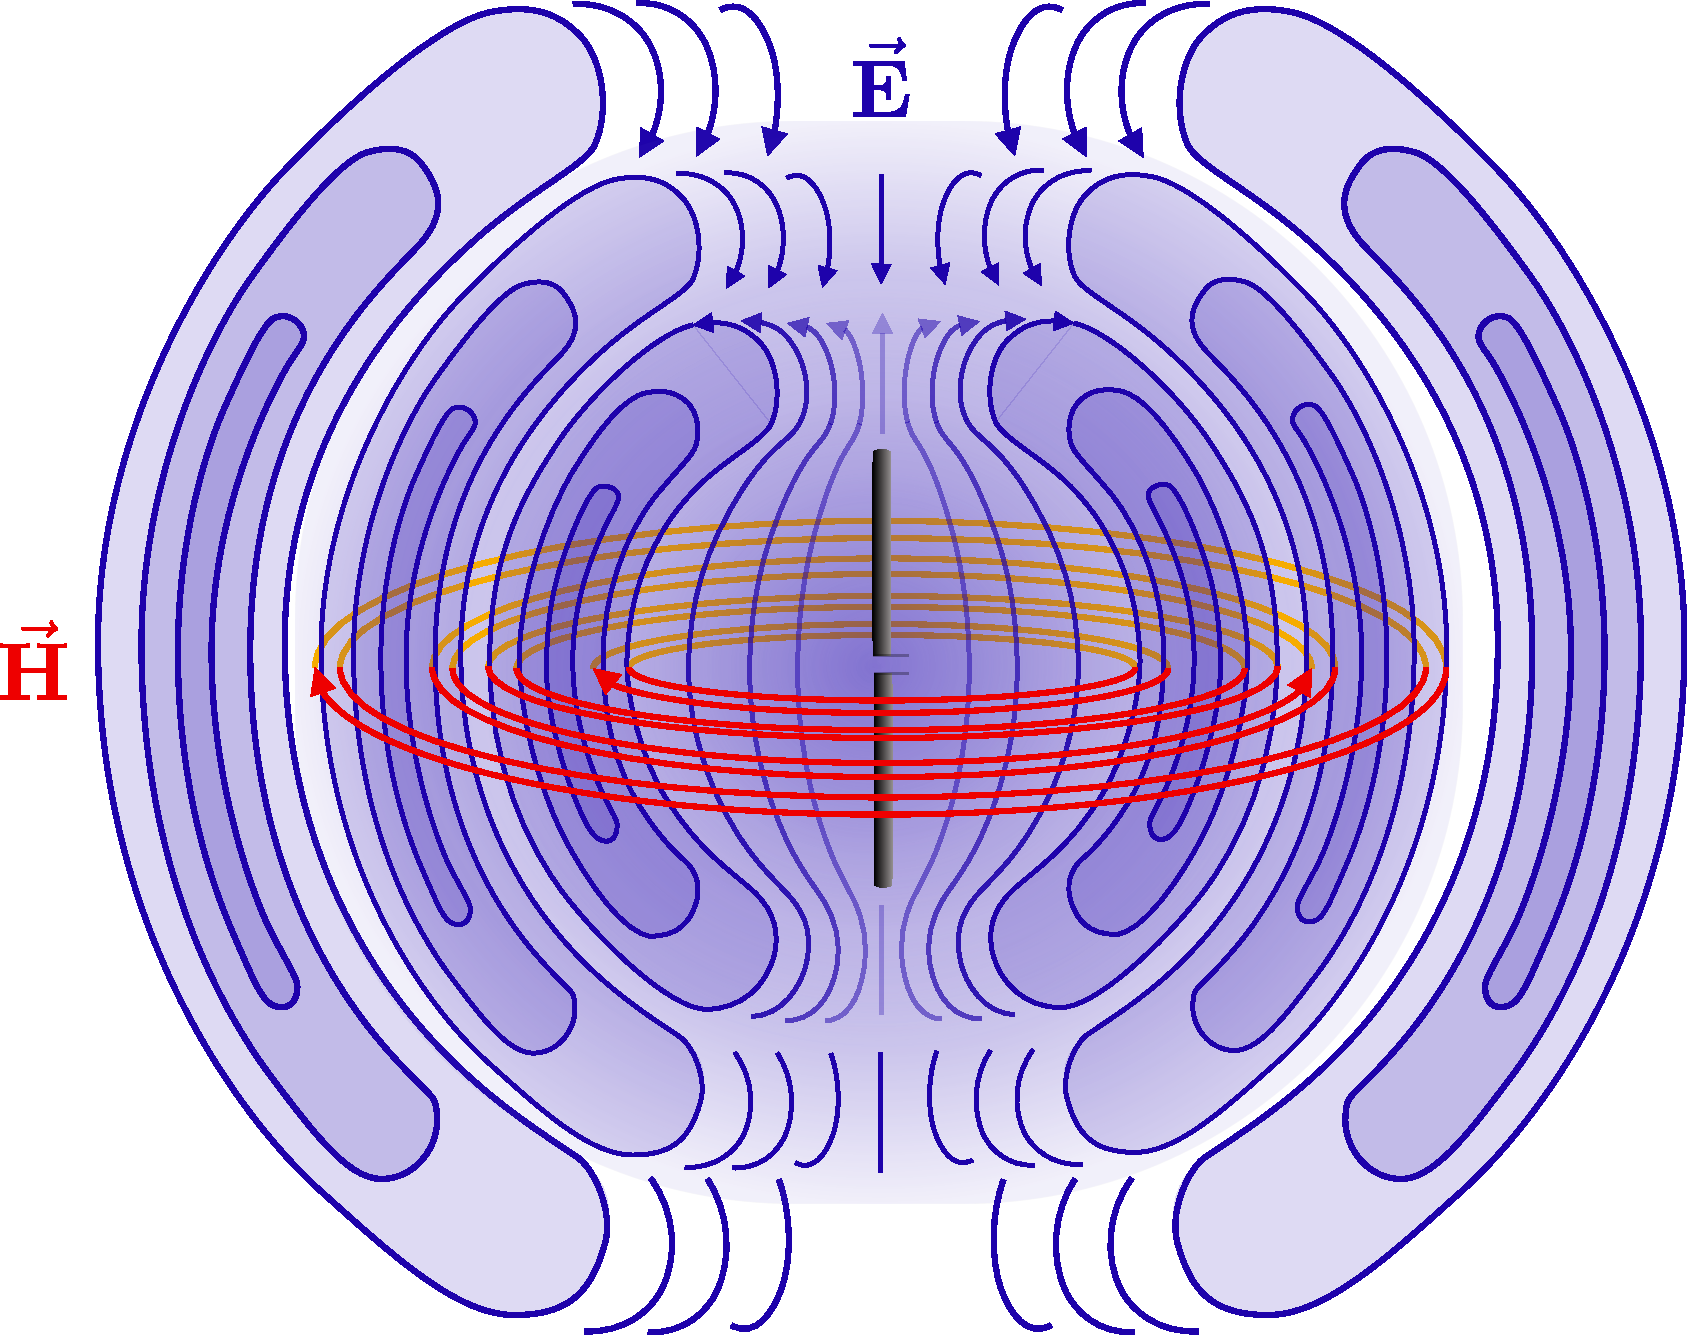
\includegraphics[width=.9\textwidth]{radiation.pdf}
      \caption{Antenna Radiation Mechanism}
    \end{figure}
      \end{column}%
\end{columns}
\end{frame}

\begin{frame}[fragile]
  \frametitle{Finding the Antenna Fields}
\begin{outline}
  \1 There are mainly two ways to find the radiated fields from a given current distribution
\end{outline}
\begin{figure}
  \centering
          {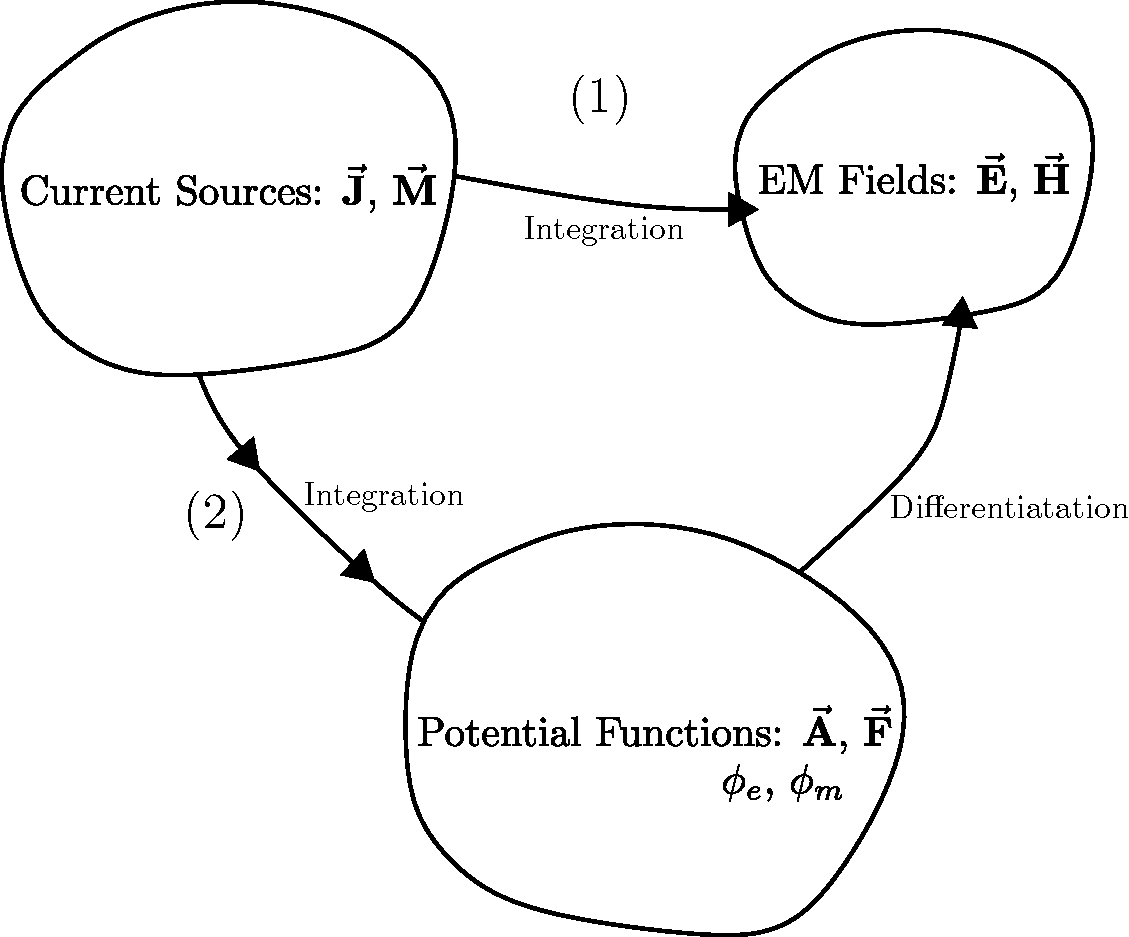
\includegraphics[width=.6\linewidth]{calculation.pdf}
        \label{fig:aug_fields}}
        \caption{Two ways to find the radiated EM fields}
\end{figure}
\end{frame}


\begin{frame}
  \frametitle{Auxiliary Potential Functions}
  \begin{outline}
    \1 Solving EM fields directly using the Maxwell's equations is often very difficult, especially in the spatial domain
    \1 The introduction of scalar ($\va{\phi}$) and vector $\va{A}$ potential functions simplify the process
    \1 We start from the fact:
    \2 Magnetic field is divergence-less ($\div \va{B} = 0$). We can therefore, say that:
  \end{outline}
  \begin{align*}
    \div \curl \va{A} \equiv 0 \\
    \Rightarrow \va{H} &= \frac{1}{\u} \curl \va{A}
  \end{align*}
  We can write the Ampere's law as:
  \begin{align*}
    \curl \va{E} &= - \j \O \u \va{H} = \j \O \curl \va{A} \\
    \curl \left (\va{E} + \j \O \va{A} \right) &= 0
  \end{align*}
\end{frame}

\begin{frame}
  \frametitle{Auxiliary Potential Functions - contd.}
  Knowing that the $\curl (-\grad \phi) \equiv 0 $, we set:
  \begin{align*}
    \va{E} + \j \O \va{A} &= -\grad \phi \\
    \va{E} &= -\grad \phi - \j \O \va{A}
  \end{align*}
\begin{outline}
  \1 $\phi$ is the electric scalar potential and its a function of position.
  \1 If we know $\va{A}$ and $\phi$, we can find $\va{E}$ and $\va{H}$
\end{outline}
\end{frame}


\begin{frame}
  \frametitle{How to find the potential functions}
  
  \begin{outline}
    \1 We still need to figure out how to find the potentials,   $\va{A}$ and $\phi$ for a given current density $\va{J}$.
    \1 For this we move back to the Maxwell's equations and find a relationship
  \end{outline}

  \begin{align*}
     \curl \va{H} &= \j \O \E \va{E} + \va{J} \\
     \curl \left( \curl \va{A} \right) &= \j \O \u \E \va{E} + \u \va{J} \\
     \curl \curl \va{A} &= \j \O \u \E \left(-\j \O \va{A} - \grad \phi \right) + \u \va{J}
  \end{align*}
\end{frame}

\begin{frame}
    \frametitle{Finding fields through potential functions}  
  Continuing and using the vector identity, 
  $\curl \curl \va{A} = \grad ( \div  \va{A} - \laplacian \va{A})$
  and rearranging, we get,
  \begin{align*}
    \laplacian \va{A} + \O^2 \u \E \va{A} &= -\u \va{J} + \grad (\div \va{A} +  \j \O \u \E \phi) 
  \end{align*}

The solution is complete by defining $\va{A}$ in terms of $\phi$ through the Lorentz gauge, 
\begin{align*}
  \div \va{A} &= - \j \O \u \E \phi
\end{align*}
\end{frame}


\begin{frame}
  \frametitle{Summary - The potential function}
  \begin{outline}
    \1 Given an electric current density $\va{J}$
    \1 Solve for the magnetic vector potential $\va{A}$
    \2 Solve for $\va{E}$ and $\va{H}$
  \end{outline}
  There are some assumptions in this method, namely:
  \begin{outline}
    \1 The space is homogeneous (only one material)
    \1 The magnetic current density $\va{M}$ is zero.
  \end{outline}
\end{frame}

  



\end{document}
